\chapter{Validation}
\label{validation}
In this last chapter, we summarize our validation of RAPID, showing that the system meets Chapter~\ref{requirements}'s critical requirements, correctly uses the concepts and technologies outlined in our Background, and is efficient enough for real use in the future.

We made two primary contributions: 1) guidelines and findings for API developers---at this point, Francis---validating our data model and overall system design and 2) performance testing results for common operations.

\section{Functionality}
RAPID includes a geospatial data model as well as file parsing and querying capabilities. We must, therefore, verify that RAPID's design meets its specification and that our codebase parses, stores, queries, and outputs geospatial data correctly. These are particularly prudent, as RAPID's entire purpose is to enable portability and interchangeability for \textit{external} partners and \textit{future} developers.

Our example setup between ABC Pipeline Co. and XYZ Operations is a relatively complete case study, showing real class instances and relationships. By showing the models and implementation patterns in Chapter~\ref{design} that support that needed functionality, it should be apparent that RAPID completely and successfully meets our system requirements from Chapter~\ref{requirements}.

Even though our model is, hopefully, convincing on its own, we worked with another student developer, Kishan Patel, to integrate a web application with RAPID for further validation. We call this software \textit{RAPID UI}, which visualizes spatial entities and our organization of data (Features in DataLayers, DataLayers grouped into GeoViews).

Our peer developer, Patel, had to become acquainted with basic geospatial concepts and client-side libraries, but our contributions to RAPID were significant and successful enough that he was able to create a sensible UI using our most important API calls. Second, being able to visualize our data---both geographic geometries and accompanying properties---we literally see that data makes it through RAPID, from beginning to end, as expected. As an additional nicety, we share and visualize several datasets with RAPID UI that were recently recommended by pipeline operating partners.

Francis describes our work with Patel in-depth---she worked with him to design and fully test REST calls---but please see the short following summary, which outlines our expectations and findings for RAPID UI (focusing on the data model's role)~\cite{Francis}. A screenshot of the interface is shown in Figure~\ref{fig:rapidui}.

\begin{itemize}
\item A primary goal in researching GIS standards and technologies was to ensure RAPID operates as expected when handling (rather finicky) geospatial data. Therefore, we set up several sample DataLayers (from GeoJSON and Shapefiles) for RAPID UI to attempt retrieving and visualizing. In particular, we had the goal of requiring as little custom UI logic as possible---relying instead upon pre-built GIS tools.

Patel and Francis ensure RAPID UI could properly request data and handle GeoJSON responses through the API (using common HTTP libraries in Python and JavaScript). After RAPID UI fetches standardized files, using particular geospatial libraries \textit{should and does} let the application parse and visualize our data in one step.

\begin{figure}[ht]
    \centering
    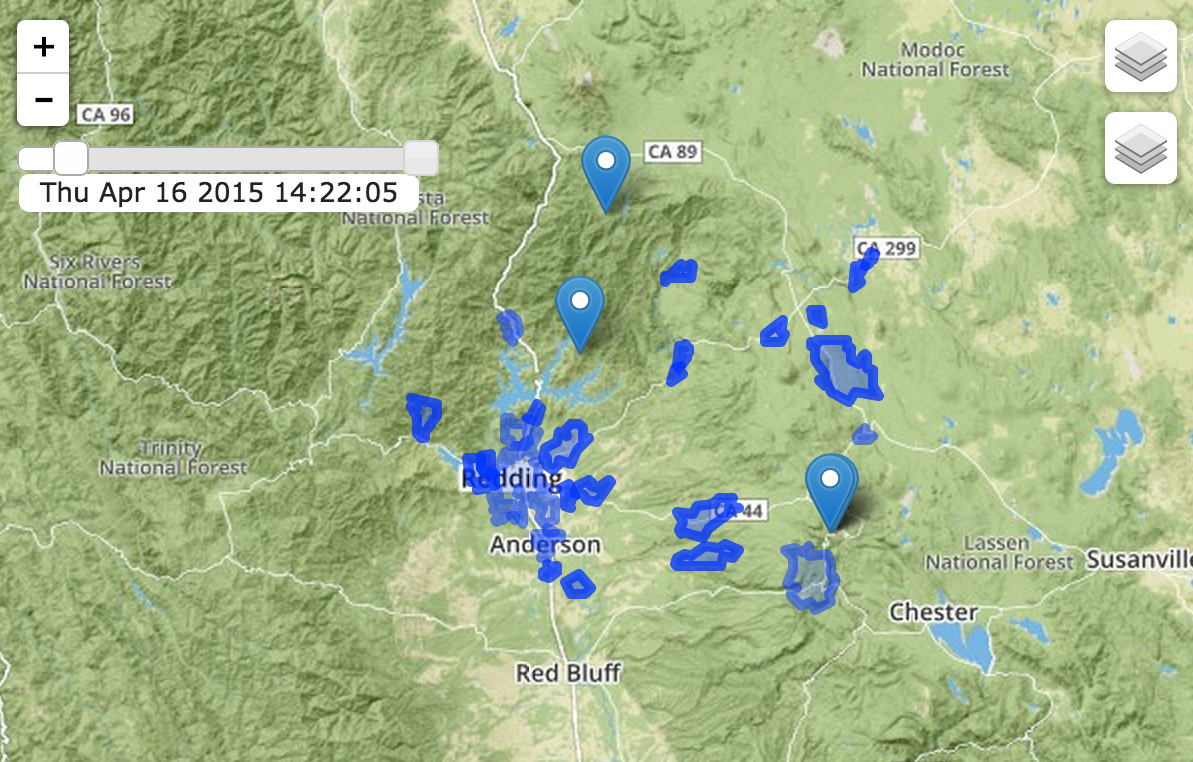
\includegraphics[width=0.84\textwidth]{figures/rapidui.png}
    \caption{RAPID UI screenshot showing two DataLayers' Features in a Shasta County GeoView.}
    \label{fig:rapidui}
\end{figure}

\item Aside from visualizing correctly-shaped and -placed geospatial Features, we had to count on RAPID UI retrieving and displaying relationships between GeoViews, DataLayers, and Features. Patel, using RAPID's JSON responses (designed by Francis), displays available GeoViews in RAPID UI, letting users switch between them and their DataLayers. That is, users can observe and analyze whichever datasets they need at that time.

\item Last, RAPID UI incorporates RAPID's geospatiotemporality by filtering data by time. For example, users can switch between days of a single month to see which Features are generated or applicable on which days.

This characteristic is demonstrably useful: out-of-date Features can be imported alongside recent data that is of much more interest. Operators frequently value hazard and encroachment \textit{prevention}, using the most up-to-date information~\cite{Dunning2013}.
\end{itemize}

\section{Performance}
The previous section shows that, given our data model and business logic, RAPID operates properly; we now use this section to highlight our core data model's performance, showing that it is an efficient foundation for future additions. We point out specific interface actions that typify DSS work and compare their runtimes.\footnote{Performance testing spatial schemas and source code could be a thesis to itself. Here, we cast a wide net, but still tackle our most visible and potentially-taxing operations.}

Spatial Feature querying is RAPID's main bottleneck. During region-specific lookups (like with GeoViews), the system must filter each Feature in a DataLayer based on spatial calculations. Automatic spatial indexing in PostGIS amortizes this, but the process is still more demanding than \texttt{SELECT} statements using one indexed unique identifier.\footnote{GeoDjango (by default) creates \textit{bounding box} indexes in PostGIS with R-Trees (see the \texttt{CREATE TABLE} and \texttt{CREATE INDEX} statements in Figure~\ref{fig:sql}).}

To study RAPID's spatial querying, we run several performance tests. One high-reaching goal for the system's future is to manage and fetch data for a whole continent; however, we just as likely expect some customers to work with smaller numbers of Features. Therefore, we test three dataset sizes, each separated by a multiplication factor of 100 Features: small (10), medium (1,000), and large (10,000).

Because the number of coordinates pairs can be orders of magnitudes different, we test spatial filtering on both Polygons and Points. Our Point dataset uses the previously-discussed USGS earthquake data---spanning the entire globe---and we specify Shasta County (in northern California) as a region of interest for filtering. Although we also use Shasta County to cull our Polygon dataset, we use United States cities for the Feature geometries. We perform each query three times and average the runtimes. See the results in Table~\ref{table:tests}.

\begin{table}
\centering
    \begin{tabular}{ |l|l|l|l|l|l| }
        % \multicolumn{4}{ |c| }{Example datasets} \\
        \hline
        Dataset & Size & Best & Middle & Worst & Average\\
        \hline
        \multirow{3}{*}{Points}
         & Small & 0.003 & 0.003 & 0.003 & 0.003 \\ \cline{2-6}
         & Medium & 0.007 & 0.007 & 0.008 & 0.007 \\ \cline{2-6}
         & Large & 0.055 & 0.056 & 0.057 & 0.056 \\ \hline
        \multirow{3}{*}{Polygons}
         & Small & 0.002 & 0.002 & 0.002 & 0.002 \\ \cline{2-6}
        & Medium & 0.012 & 0.012 & 0.012 & 0.012 \\ \cline{2-6}
         & Large & 0.393 & 0.395 & 0.398 & 0.395 \\ \hline
    \end{tabular}
    
    \caption{Performance testing results (measured in seconds).}
    \label{table:tests}
\end{table}

Two characteristics are especially notable: 1) taken as a whole, spatial queries are efficient, and 2) spatial queries scale well---not showing exponential growth, as one might expect. PostGIS indexes and \texttt{WITHIN} queries are constructed such that, even with hundreds of thousands of table rows (and, for polygon geometries, encoded data for tens of millions of data points), GeoView results can be evaluated in under half a second on commodity hardware.\footnote{These test results come from running the test queries on our development server---a virtual machine with 1 GB RAM and a 2.5 GHz CPU.} In addition, increasing the number of Features in a DataLayer by two orders of magnitude only shows lookups slowing down by, at most, thirty-three times (usually not even ten times).


\section{Unit testing discussion}
The following recommendations could be used to further validate RAPID with a thorough unit test suite.\footnote{On the back end, RAPID could use the Python's built-in testing module, \texttt{unittest}~\cite{DjangoTesting}} Once each required field for geospatial features is located for each possible input and output, exhaustive unit tests can ensure that fields in an input format can be converted to the corresponding fields in any output format. In the event storage or conversion fails, unit tests for the following components would reveal where and why:

\begin{itemize}
\item Writable and parseable digital format like GeoJSON or Shapefile.
\item In-memory objects (our own models or GEOSGeometry objects\footnote{We discussed GEOSGeometry briefly in Section~\ref{sec:export}.}).
\item WKT or GeoJSON---abstract text formats for geospatial features.
\item Abstract data persisted in PostGIS.
\end{itemize}

Data can move up and down that list; each step and transition (all outlined in Chapter~\ref{design}), should be considered a data integrity checkpoint that deserves a unit test. For instance, a Polygon made up of coordinate pairs (0, 0), (0, 10), and (10, 0) still needs to have the same meaning---a triangle with those three points---no matter its format or original location.

GeoJSON, Shapefiles, Python objects, WKT, and PostGIS data structures can all be inspected to see that the same data is contained in each. If not, it was misshaped somewhere along the line---traceable with these ``checkpoints.''